\icode{E-MD-CA-L2-261111-004}
如图，质量 \(M =\) \,\qty{4}{kg}的木板长 \(L =\) \,\qty{4}{m}，静止在光滑的水平地面上，其水平上表面左端静置一个质量 \(m =\) \,\qty{2}{kg}的小滑块（可视为质点），小滑块与板间的动摩擦因数 \(\mu = 0.2\)。从某时刻开始，用水平力 \(F =\) \,\qty{10}{N}一直向右拉滑块，直至滑块从木板上滑出。\(g\) 取\qty{10}{m/s^2}。求：
\begin{enumerate}
	\item 滑块加速度 \(a_1\) 的大小；
	\item 滑块离开木板时速度 \(v\) 的大小。
\end{enumerate}

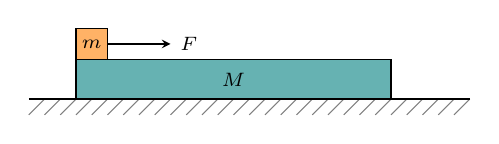
\begin{tikzpicture}[>=stealth,font=\scriptsize]
	\draw[fill=teal!60] (0,0) rectangle(4,.5)node[midway]{\(M\)};
	\draw[fill=orange!60] (0,.5) rectangle(.4,.9)node[midway]{\(m\)};
	\draw[->] (.4,.7)--++(.8,0)node[right]{\(F\)};
	\foreach \x in {-.6,-.4,...,5}
		\draw[gray] (\x,-.2)--++(.2,.2);
	\draw[thick] (-.6,0)--(5,0);
\end{tikzpicture}
\begin{answer}
	（1）\qty{3}{m/s^2}（2）\qty{6}{m/s}
\end{answer}